\section{Results and discussion}\label{sec:results}

In this section, we detail the findings of our study.  We remind the reader that our main goal with this study is the detection of potential blindspots existing in current mining sandbox approaches when detecting malware. To this end, we hypothesize the presence of two major blindspots - path taken by the app from the entry point to a sensitive API, and the differences in manifest file of repackaged apps. In Section~\ref{sec:testGeneration}, we summarize the results of our study that estimates the performance of the test generation tools for mining Android  Sandboxes, in terms of malware detection. Section \ref{sec:path} presents the results of our study analysing the impact of path on sandbox approaches to detect malware thereby answering R1, and Section~\ref{sec:manifest} presents the results of our study analysing the impact of modified manifest files on sandbox approaches to detect malware thereby answering R2. Section~\ref{sec:implications} presents some insights gained from the overall study and their potential implications.

\subsection{Effectiveness of Test generation tools on Detecting Malicious apps}\label{sec:testGeneration}

\kn{In this subsection, are we simply reproducing the results of existing papers. Because as far as I understand, tools like DroidBOT etc. were evaluated by simply comparing the sensitive APIs call. I am guessing here our contribution is to evaluate it on the larger dataset. I have given it a shot, please keep me posted if this is correct.}

In this section, we describe the results of reproducing the state of the art android sandbox approaches on the new dataset of $824$ app pairs. We perform this experiment to ensure our analysis of the blind spots are done in the same playing field. 
Firstly, given a pair of apps, we first execute each version of app using each test generation tool for three minutes. After execution, DroidXP produces a dataset with the sensitive APIs that both app versions call. We consider that a test generation tool could construct a sandbox able to detect a specific malware, if a particular sensitive API is called only be the malicious version of the app. This check is done using DroidXP. 

Then, we generate a report that includes a set of observations like the tool name, the number of the repetition (in the range [1..3])\kn{Isnt the number of repetitions always 3?}, and a boolean value indicating whether or not the malware has been identified. Figure~\ref{fig:accuracy} presents the result of each individual test generation tool in detecting malware at our data set (824 app pair).

\kn{In the following paragraph, two things are unclear to me. 1. why only for malware detected by all. Why dont we do this observation for all pairs. I dont get how high score will contribute to false positives and vice versa.}
Among the malware detected by all test generation tools, we also observe their similarity score as defined in Section~\ref{sec:similarity}. We choose  not to discard any malware based on a selected threshold, since this could lead to false positives and false negatives. For example, if we use a high similarity score for selected malware, we will have a low false positive and high false negative. On the other hand, a low similarity score brings high false positives and low false negatives. Zhou et al.\cite{DBLP:conf/codaspy/ZhouZJN12} mention the threshold of 70\% as a good balance to infer whether an app is repackaged or not. To this end, our results also present how many detected malware are above and below this threshold (70\%), for each tool.\newline
\newline
\textbf{Droidbot:} When using Droidbot to build sandbox, our results present that it could detect a total of $677$ malware among $824$ app pairs (82.16\%). Among tools used in our study, Droidbot was the most efficient in terms of the detection of apps with malicious behavior validating the results of other works~\cite{DBLP:conf/wcre/BaoLL18}\cite{DBLP:journals/jss/CostaMMSSBNR22} that observed that Droidbot detected the largest number of malicious apps. Among all malicious apps detected, $347$ have a similarity score below 70\% and $330$ above.\newline
\newline
\textbf{Monkey}, the standard test generation tool from the Android SDK  produced a sandbox that detected $527$ malware out of the dataset (63.95\%). It created the second best efficient sandbox in our study, although it implements the most basic random test strategy~\cite{DBLP:conf/icst/WetzlmaierRP16}\cite{DBLP:conf/kbse/ChoudharyGO15}. $288$ malware detected has similarity score below 70\% and $239$ above.   \newline
\newline
\textbf{Droidmate2:} Droidmate was designed with an explicit goal of monitoring calls to a set of sensitive APIs defined in the framework AppGuard~\cite{DBLP:conf/esorics/BackesGHMS13}.  Droidmate sandbox detected $414$ malicious apps (50.24\%); only a little more than half of the dataset. Among malware detected, $224$ have a score below 70\% and $190$ above.\newline
\newline
\textbf{Humanoid:}  The tool that emulates realistic users had the worst performance in comparison to others. Since Humanoid creates human-like test inputs, based on a learned model, we believe that in a simulated environment, its ability to generate test inputs is impaired. The resulting sandbox identified 401 malicious apps in our dataset (48.66\%), less than half of the dataset. From the perspective of the similarity threshold (70\%), it was the only tool that had lesser malware with a score below 70\% ($197$) than the ones above 70\% ($204$).


\begin{obs}{1}{}
   \kn{Here we need to add some final take aways of the reproduction study}
 \end{obs}

\begin{figure}[ht]
\centering
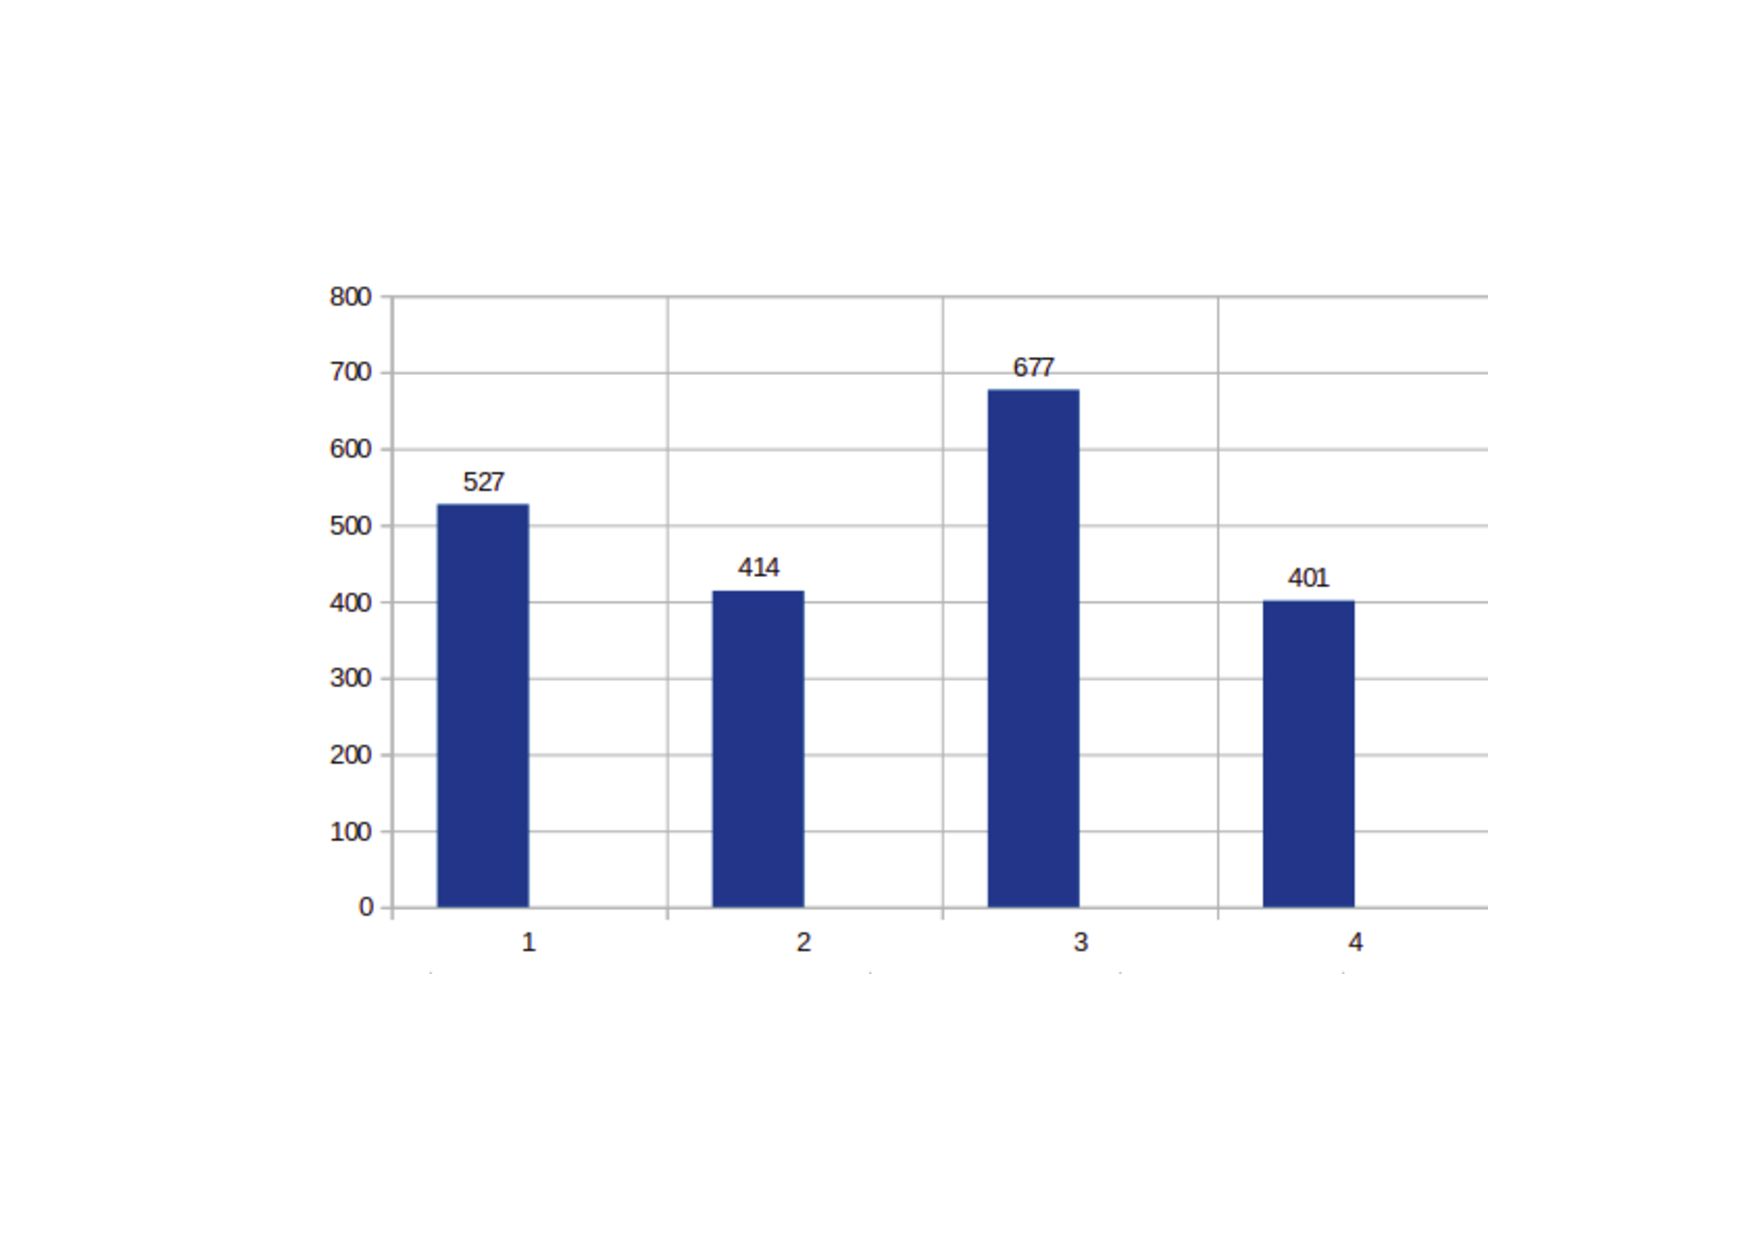
\includegraphics[scale=0.3]{images/accuracy.pdf}
\caption{Accuracy of each test generator tool on malware detection.}
 \label{fig:accuracy}
\end{figure}

\subsection{Path Analysis}\label{sec:path}

In this section, we describe the results of our investigation on how the path from the entry point to the sensitive API could impact the accuracy of sandbox approaches detecting android malware. To this end, we collect the call graphs of each test generation tool using \emph{Logcat}. First, we make a filter to collect just the paths between the app'S entry point and the call to any sensitive methods as defined framework AppGuard.

Finally, with callgraph from both the benign and malicious app versions, we we spot differences between any paths. For this section, we choose to investigate only app pairs that were not detected by  the sandbox approaches as it sheds light on the blind-spots. Our results show that it is possible to improve malware detection if we also consider the path between app's entry point and calls to sensitive call.

Table~\ref{tab:pa} summarizes the results of this investigation. The column \textbf{Execution (NID)} shows the number of undetected malwares. The column  \textbf{Path Different (PD)} shows the number of app pairs (among the undetected ones) that have different paths from the entry point to the sensitive method call. The column \textbf{Improvement \%} shows how much the malware detection of each tool could have been potentially improved if we considered the path (calculated using ~\eqref{improve})


\begin{table}[ht]
  \caption{Summary of the results of path analysis. }
  \centering
  \begin{small}
 \begin{tabular}{lrrr}
   \toprule
   Tool & Execution (NID) & Path Analysis (PD) & Improvement (\%) \\   \midrule
   Monkey &  297 & 157 & 52.86 \\ 
   Droidmate &  410 & 259 & 63.17 \\ 
   Droidbot &  147 & 103 & 70.06 \\ 
   Humanoid &  423 & 27 & 39.71 \\ 
 \bottomrule
 \end{tabular}
 \end{small}
 \label{tab:pa}
\end{table}

\begin{eqnarray}
Improvement & = & \frac{Path Analysis (DP) \times 100}{Execution (NID)} 
\label{improve}
\end{eqnarray}

\begin{obs}{2}{}
 All test generation tools have a blind-spot when it comes to being aware of the path taken from the entry point to a sensitive API call (atleast $39\%$). Even the most successful sandbox approaches like DroidBot could have detected $70\%$ of its undetectable app pairs had it considered path as a factor. 
\end{obs}


\subsection{Manifest File Analysis}\label{sec:manifest}

In this section, we describe the results of our investigation on the impact of modified manifest files towards the accuracy of sandbox approaches. 
To this end, we check some particulars from Manifest file, that point to a likely suspicious behavior. In section \ref{sec:manifestAnalysis}, we illustrated that an automatic hacking script could inject duplicated permission and actions into the Manifest file. We looked out for such modifications in the malware that went undetected by the test generation tools. We also check if among these apps, there were requests to new permissions, that were not initially requested by the benign version, or if there were excessive requests for permissions in the malicious version's manifest files. Table~\ref{tab:mfa} summarizes our results. 

\begin{table}[ht]
  \caption{Manifest File with duplicate code.}
  \centering
  \begin{small}
 \begin{tabular}{lccccc}
   \toprule
   Tool & (NID) & (DP) & (DA) & (DP or DA) & (DP and DA) \\   \midrule
   Monkey &  297 & 36 & 44 & 62 & 18 \\ 
   Droidmate &  410 & 48 & 63 & 91 & 20 \\ 
   Droidbot &  147 & 18 & 25 & 36 & 7 \\ 
   Humanoid &  423 & 51 & 61 & 91 & 21 \\ 
 \bottomrule
 \end{tabular}
 \end{small}
 \label{tab:mfa}
\end{table}

The column (NID) indicates the number of malware that went undetected during our first study ( same as Table~\ref{tab:pa}'s Execution NID column). The second column (DP) indicates how many Manifest files had duplicated permission. Column (DA) denotes the number of malware with the duplicated actions in their manifest file.

A duplicate request to permission in a malicious version's manifest file should have been performed by a script.  Droidbot and Humanoid could have detected $91$ of their undetectable malwares had they considered duplicate permissions or actions in their detection strategy.  

Interestingly, among all app pairs  that contain both a duplicate permission and action(69 app pairs), just $4$ have the similarity score above 70\%, $2$ from Monkey, $1$ from Droidmate, and $1$ from Humanoid. Other app pairs with very suspicious Manifest file, have a high similarity score, which indicates that it would indeed be difficult to detect using a basic sandbox approach. 

Finally, we investigate how many app pairs request a suspicious amount of permissions. Past works indicate that a benign Android app normally requests on average $4$ permission, while a malicious apps version requests a median number of $7$ permission\cite{DBLP:conf/soups/FeltHEHCW12}\cite{DBLP:journals/tifs/0029LBKTLC17}. To this end, we observe how many app pairs have more than a delta of $3$ permission requests in comparison with the benign version. Table~\ref{tab:mp} presents the results.

\begin{table}[ht]
  \caption{Manifest File with suspiscious amounts of permission requests.}
  \centering
  \begin{small}
 \begin{tabular}{lccc}
   \toprule
   Tool & (MP) & (DP) & (NDP) \\   \midrule
   Monkey &  10 & 8 & 2 \\ 
   Droidmate &  11 & 8 & 3 \\ 
   Droidbot &  3 & 1 & 2 \\ 
   Humanoid &  15 & 11 & 4 \\ 
 \bottomrule
 \end{tabular}
 \end{small}
 \label{tab:mp}
\end{table}

The second column (MP) present how many app pairs not detected by each test generation tool, have other suspicious number of permission requests ($4$ or more) in their Manifest file. Third and fourth columns (DP)(NDP) presents how many app pairs out of these contain duplicated permission or not respectively. As we can see, most of app pair that have excessive permission request, also have duplicated permission in your code. 


\begin{obs}{3}{}
 We can conclude that all test generation tools  would have had better accuracy had they considered the modifications to manifest file in their analysis. 
\end{obs}

\subsection{Implications}\label{sec:implications}